\documentclass{article}

\usepackage{pandekten}
\usepackage{dashrule}

\makeatletter
\newcommand*{\shifttext}[1]{%
  \settowidth{\@tempdima}{#1}%
  \hspace{-\@tempdima}#1%
}
\newcommand{\plabel}[1]{%
\shifttext{\textbf{#1}\quad}%
}
\newcommand{\prule}{%
\begin{center}%
\hdashrule[0.5ex]{.99\linewidth}{1pt}{1pt 2.5pt}%
\end{center}%
}

\makeatother

\newcommand{\minusbaseline}{\abovedisplayskip=0pt\abovedisplayshortskip=0pt~\vspace*{-\baselineskip}}%

\setlength{\parindent}{0pt}

\title{Assignment 5}
\author{Ze Chen}

\begin{document}

\maketitle

% \bibliographystyle{plain}
% \bibliography{main}

\plabel{1}%
The Feynman rules are given below.
\begin{center}
    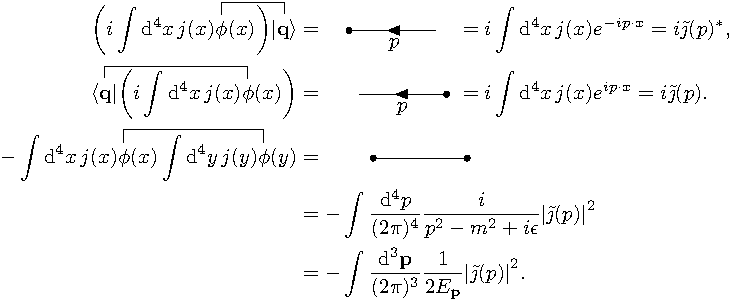
\includegraphics{img/problem-1/leg.pdf}
\end{center}
Let $\displaystyle C_m = \frac{(2m)!}{m!2^m}$ be the number of contractions on $\phi(x_1) \cdots \phi(x_{2m})$.
Now we evaluate
\begin{align*}
    &{\phantom{=}}\mel**{\vb{p}_1,\cdots,\vb{p}_n}{T\qty{\exp[i\int \dd[4]{x} j(x)\phi_I(x)]}}{0} \\
    &= \raisebox{-.5\height+2pt}{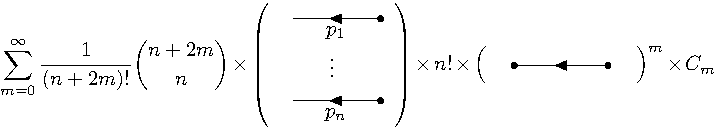
\includegraphics{img/problem-1/sum.pdf}} \\
    &= \sum_{m=0}^\infty \frac{1}{m!} i^n \tilde{\jmath}(p_1) \cdots \tilde{\jmath}(p_n) \qty(-\frac{1}{2}\int \frac{\dd[3]{\vb{p}}}{(2\pi)^3}\frac{1}{2E_{\vb{p}}}\abs{\tilde{\jmath}(p)}^2)^m \\
    &= i^n \tilde{\jmath}(p_1) \cdots \tilde{\jmath}(p_n) \exp(-\frac{1}{2}\int \frac{\dd[3]{\vb{p}}}{(2\pi)^3}\frac{1}{2E_{\vb{p}}}\abs{\tilde{\jmath}(p)}^2).
\end{align*}
Taking the density of states into account, we find
\begin{align}
    \notag &\phantom{{}={}} P(\vb{p}_1,\cdots,\vb{p}_n) \dd[3]{\vb{p}_1} \cdots \dd[3]{\vb{p}_n} \\
    \notag &= \abs{\mel**{\vb{p}_1,\cdots,\vb{p}_n}{T\qty{\exp[i\int \dd[4]{x} j(x)\phi_I(x)]}}{0}}^2 \frac{\dd[3]{\vb{p}_1}}{(2\pi)^3 2E_{\vb{p}_1}} \cdots \frac{\dd[3]{\vb{p}_n}}{(2\pi)^3 2E_{\vb{p}_n}} \\
    \label{eq:pj0} &= \abs{\tilde{\jmath}(p_1)}^2 \cdots \abs{\tilde{\jmath}(p_n)}^2 \exp(-\int \frac{\dd[3]{\vb{p}}}{(2\pi)^3}\frac{1}{2E_{\vb{p}}}\abs{\tilde{\jmath}(p)}^2) \frac{\dd[3]{\vb{p}_1}}{(2\pi)^3 2E_{\vb{p}_1}} \cdots \frac{\dd[3]{\vb{p}_n}}{(2\pi)^3 2E_{\vb{p}_n}}.
\end{align}
Let
\[ \lambda = \int \frac{\dd[3]{\vb{p}}}{(2\pi)^3}\frac{1}{2E_{\vb{p}}}\abs{\tilde{\jmath}(p)}^2. \]

\plabel{(a)}%
This is just
\[ U(+\infty,-\infty) = T\qty{\exp[-i\int_{-\infty}^\infty \dd{t'} H'_I(t')]} \]
for the case
\[ H'_I(t) = \int \dd[3]{\vb{x}} (-j(t,\vb{x}) \phi_I(t,\vb{x})). \]

\plabel{(b, c)}%
This is just \cref{eq:pj0} applied to the final state $\bra{0}$.
\begin{align*}
    P(0) = \abs{\mel**{0}{T\qty{\exp[i\int \dd[4]{x} j(x)\phi_I(x)]}}{0}}^2 &= \exp(-\int \frac{\dd[3]{\vb{p}}}{(2\pi)^3}\frac{1}{2E_{\vb{p}}}\abs{\tilde{\jmath}(p)}^2) \\
    &= e^{-\lambda} \approx 1 - \lambda.
\end{align*}

\plabel{(d)}%
This is just \cref{eq:pj0} applied to the final state $\bra{\vb{k}}$.
\[ P(\vb{k}) \dd[3]{\vb{k}} = \abs{\tilde{\jmath}(k)}^2 \exp(-\int \frac{\dd[3]{\vb{p}}}{(2\pi)^3}\frac{1}{2E_{\vb{p}}}\abs{\tilde{\jmath}(p)}^2) \frac{\dd[3]{\vb{k}}}{(2\pi)^3 2E_{\vb{k}}}. \]

\plabel{(e)}%
With \cref{eq:pj0} and taking symmetry factor $1/n!$ into account we find
\begin{align*}
    P(n) &= \frac{1}{n!} \int P(\vb{p}_1,\cdots,\vb{p}_n) \dd[3]{\vb{p}_1} \cdots \dd[3]{\vb{p}_n} = \frac{1}{n!} \lambda^n \exp(-\lambda).
\end{align*}

\plabel{(f)}%
\begingroup\minusbaseline
\begin{align*}
    \sum_{n=0}^\infty P(n) &= e^{-\lambda} \sum_{n=0}^\infty \frac{1}{n!}\lambda^n = \exp(-\lambda) \exp(\lambda) = 1, \\
    \langle N \rangle = \sum_{n=0}^\infty nP(n) &= e^{-\lambda} \sum_{n=0}^\infty \frac{1}{n!}\lambda^{n+1} = \lambda \exp(-\lambda) \exp(\lambda) = \lambda, \\
    \langle N^2 \rangle = \sum_{n=0}^\infty n^2P(n) &= e^{-\lambda} \sum_{n=0}^\infty \frac{1}{n!}(\lambda^{n+1} + \lambda^{n+2}) = \lambda + \lambda^2, \\
    \langle (N - \langle N\rangle)^2 \rangle &= \langle N^2 \rangle - \langle N \rangle^2 = \lambda.
\end{align*}
\endgroup

\prule

\plabel{2 (a)}
\begingroup\minusbaseline
\begin{align*}
    \Gamma &= \frac{1}{2m_1\abs{S}} \int \frac{\dd[3]{\vb{p}_2}}{(2\pi)^3 2E_2} \frac{\dd[3]{\vb{p}_3}}{(2\pi)^3 2E_3} (2\pi)^4 \delta(E_1 - E_2 - E_3) \delta^{(3)}(\vb{p}_2 + \vb{p}_3) \\
    &\phantom{{}=\frac{1}{2m_1\abs{S}} \int \frac{\dd[3]{\vb{p}_2}}{(2\pi)^3 2E_2} \frac{\dd[3]{\vb{p}_3}}{(2\pi)^3 2E_3}}{} \times \abs{\mathcal{M}((m_1,0) \rightarrow (m_2,\vb{p}_2) + (m_3,\vb{p}_3))}^2 \\
    &= \frac{1}{2m_1\abs{S}} \frac{1}{(2\pi)^2 4E_2 E_3} \int \dd[3]{\vb{p}_2} \delta(m_1 - E_2 - E_3) \\
    &{\phantom{{}=\frac{1}{2m_1\abs{S}} \frac{1}{(2\pi)^2 4E_2 E_3} \int \dd[3]{\vb{p}_2}}} {} \times \abs{\mathcal{M}((m_1,0) \rightarrow (m_2,\vb{p}_2) + (m_3,-\vb{p}_2))}^2.
\end{align*}
\endgroup

\plabel{(b)}%
\begingroup\minusbaseline
\begin{align*}
    \Gamma &= \frac{1}{2m_1\abs{S}} \frac{4\pi}{(2\pi)^2 4E_2 E_3} \int \dd{\abs{\vb{p}_2}} \abs{\vb{p}_2}^2 \delta(m_1 - E_2 - E_3) \\
    &{\phantom{{}=\frac{1}{2m_1\abs{S}} \frac{1}{(2\pi)^2 4E_2 E_3} \int \dd{\abs{\vb{p}_2}} }} {} \times \abs{\mathcal{M}((m_1,0) \rightarrow (m_2,\vb{p}_2) + (m_3,-\vb{p}_2))}^2 \\
    &= \frac{1}{8\pi m_1 \abs{S} E_2 E_3} \eval{\frac{\abs{\vb{p}_2}^2 \abs{\mathcal{M}}^2}{\abs{\vb{p}_2}/E_2 + \abs{\vb{p}_2}/E_3}}_{\eval{(E_2+E_3)}_{\vb{p}_2} = m_1} \\
    &= \frac{\abs{\vb{p}_2}}{8\pi m_1^2 \abs{S}} \abs{\mathcal{M}}^2.
\end{align*}
\endgroup

\plabel{(c)}%
If $m_1 \le m_2 + m_3$ then either $m_1 - E_2 - E_3 = 0$ has solution $\abs{\vb{p}_2} = 0$ or has no solution and therefore
\[ \int \dd{\abs{\vb{p}_2}} \abs{\vb{p}_2}^2 \delta(m_1 - E_2 - E_3) \cdots = 0. \]
$\abs{p}_2$ is obtained by solving $m_1 - E_2 - E_3 = 0$.
\[ \abs{\vb{p}_2} = \frac{\sqrt{(M^2 - (m_1+m_2)^2)(M^2 - (m_1 - m_2)^2)}}{2m_1}. \]
$\Gamma$ is evaluated above.
\[ \Gamma = \frac{\abs{\vb{p}_2}}{8\pi m_1^2 \abs{S}} \abs{\mathcal{M}}^2. \]
The dimensions of both sides are identical.
\[ \mathrm{mass}^{-1} = \frac{\mathrm{mass}}{\mathrm{mass}^{2}} \times 1. \]

\prule

\clearpage
\plabel{3}%
The Feynman rules are given below.
\begin{itemize}
    \item Propagators:
    \begin{center}
        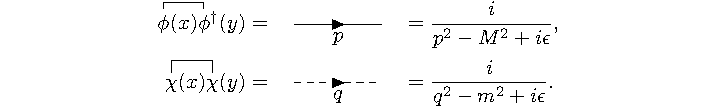
\includegraphics{img/propagator/propagator.pdf}
    \end{center}
    \item Vertices:
    \begin{center}
        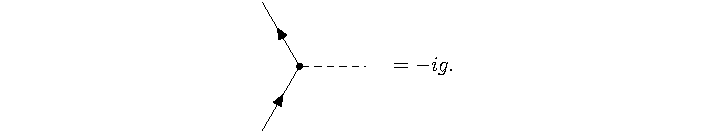
\includegraphics{img/vertex/vertex.pdf}
    \end{center}
    \item External leg contractions:
    \begin{center}
        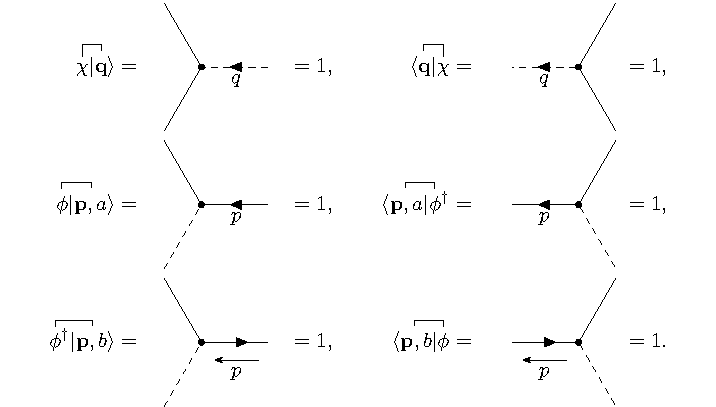
\includegraphics{img/leg/leg.pdf}
    \end{center}
\end{itemize}
\plabel{(1)}%
The $s$-channel Feynman diagram is given below.
\begin{center}
    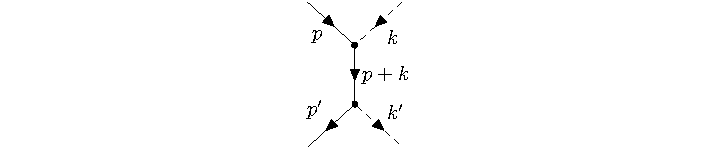
\includegraphics{img/compton/compton-s.pdf}
\end{center}
The amplitude is given by
\[ i\mathcal{M} = \frac{-ig^2}{(p+k)^2 - M^2} = \frac{-ig^2}{s^2-M^2}. \]
The $u$-channel Feynman diagram is given below.
\begin{center}
    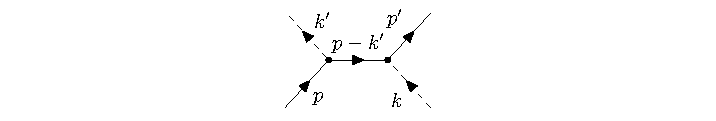
\includegraphics{img/compton/compton-u.pdf}
\end{center}
The amplitude is given by
\[ i\mathcal{M} = \frac{-ig^2}{(p-k')^2 - M^2} = \frac{-ig^2}{u^2-M^2}. \]
Summing up we find
\[ i\mathcal{M} = -ig^2\qty(\frac{1}{s^2 - M^2} + \frac{1}{u^2 - M^2}). \]

\plabel{(2)}%
The $t$-channel Feynman diagram is given below.
\begin{center}
    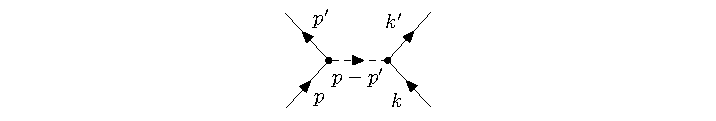
\includegraphics{img/moller/moller-t.pdf}
\end{center}
The amplitude is given by
\[ i\mathcal{M} = \frac{-ig^2}{(p-p')^2 - m^2} = \frac{-ig^2}{t^2-m^2}. \]
The $u$-channel Feynman diagram is given below.
\begin{center}
    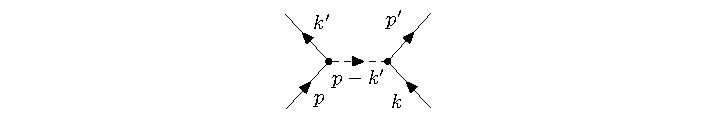
\includegraphics{img/moller/moller-u.pdf}
\end{center}
The amplitude is given by
\[ i\mathcal{M} = \frac{-ig^2}{(p-k')^2 - m^2} = \frac{-ig^2}{u^2-m^2}. \]
Summing up we find
\[ i\mathcal{M} = -ig^2\qty(\frac{1}{t^2 - m^2} + \frac{1}{u^2 - m^2}). \]
In the CM frame, the energy of each particle is $E = E_{\mathrm{cm}} / 2$, and
\begin{align*}
    t^2 - m^2 &= -2(E^2 - M^2)(1 - \cos\theta) - m^2, \\
    u^2 - m^2 &= -2(E^2 - M^2)(1 + \cos\theta) - m^2.
\end{align*}
Therefore,
\[ \abs{\mathcal{M}}^2 = g^4\qty(\frac{4 \qty(E_{\mathrm{cm}}^2+2 m^2-4 M^2)}{\qty(E_{\mathrm{cm}}^2-4 M^2)^2 \cos ^2(\theta )-\qty(E_{\mathrm{cm}}^2+2 m^2-4 M^2)^2})^2. \]
The differential cross section is given by
\begin{align*}
    \qty(\dv{\sigma}{\Omega})_{\mathrm{CM}} &= \frac{\abs{\mathcal{M}}^2}{64\pi^2 E^2_{\mathrm{cm}}} \\
    &= \frac{g^4}{4 \pi^2 E_{\mathrm{cm}}^2} \qty(\frac{ \qty(E_{\mathrm{cm}}^2+2 m^2-4 M^2)}{\qty(E_{\mathrm{cm}}^2-4 M^2)^2 \cos ^2(\theta )-\qty(E_{\mathrm{cm}}^2+2 m^2-4 M^2)^2})^2.
\end{align*}
The differential cross section is maximal at $\theta = 0$ or $\theta = \pi$.
If $m = 0$, then $\displaystyle \qty(\dv{\sigma}{\Omega})_{\mathrm{CM}} \sim \frac{1}{\sin^4 \theta}$.
The total cross section is given by
\begin{align*}
    \sigma &= \int \qty(\dv{\sigma}{\Omega})_{\mathrm{CM}} \dd{\Omega} = 2\pi \int \qty(\dv{\sigma}{\Omega})_{\mathrm{CM}} \cdot \sin\theta \dd{\theta} \\
    &= \frac{2g^4}{\pi  E_{\mathrm{cm}}^2 \left(E_{\mathrm{cm}}^2-4 M^2+2 m^2\right)} \times \\
    &\phantom{{}={}} \qty[
        2 g^4 \left(\frac{1}{E_{\mathrm{cm}}^2-4 M^2+m^2}+\frac{2 \ln \qty[\left(E_{\mathrm{cm}}^2-4 M^2+m^2\right)/m^2]}{E_{\mathrm{cm}}^2-4 M^2}+\frac{1}{m^2}\right)
    ]
\end{align*}

\plabel{(3)}%
The $s$-channel Feynman diagram is given below.
\begin{center}
    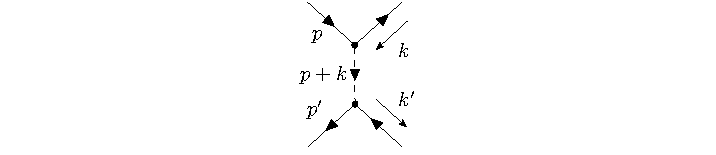
\includegraphics{img/bhabha/bhabha-s.pdf}
\end{center}
The amplitude is given by
\[ i\mathcal{M} = \frac{-ig^2}{(p+k)^2 - m^2} = \frac{-ig^2}{s^2-m^2}. \]
The $u$-channel Feynman diagram is given below.
\begin{center}
    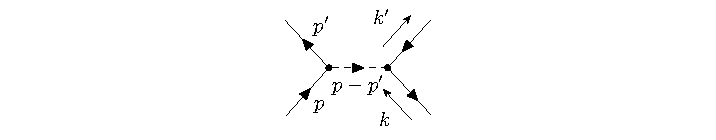
\includegraphics{img/bhabha/bhabha-t.pdf}
\end{center}
The amplitude is given by
\[ i\mathcal{M} = \frac{-ig^2}{(p-p')^2 - m^2} = \frac{-ig^2}{t^2-m^2}. \]
Summing up we find
\[ i\mathcal{M} = -ig^2\qty(\frac{1}{s^2 - m^2} + \frac{1}{t^2 - m^2}). \]
In the CM frame, the energy of each particle is $E = E_{\mathrm{cm}} / 2$, and
\begin{align*}
    s^2 - m^2 &= 4E^2 - m^2, \\
    t^2 - m^2 &= -2(E^2 - M^2)(1 - \cos\theta) - m^2.
\end{align*}
Therefore,
\[ \abs{\mathcal{M}}^2 = g^4\qty(\frac{1}{4E^2 - m^2} - \frac{1}{2(E^2 - M^2)(1 - \cos\theta) + m^2})^2. \]
The differential cross section is given by
\begin{align*}
    \qty(\dv{\sigma}{\Omega})_{\mathrm{CM}} &= \frac{\abs{\mathcal{M}}^2}{64\pi^2 E^2_{\mathrm{cm}}} \\
    &= \frac{g^4}{64 \pi^2 E_{\mathrm{cm}}^2} \qty(\frac{1}{E_{\mathrm{cm}}^2 - m^2} - \frac{1}{2(E_{\mathrm{cm}}^2/4 - M^2)(1 - \cos\theta) + m^2})^2.
\end{align*}
The differential cross section is maximal at $\theta = \pi$.
The total cross section is given by
\begin{align*}
    \sigma &= \int \qty(\dv{\sigma}{\Omega})_{\mathrm{CM}} \dd{\Omega} = 2\pi \int \qty(\dv{\sigma}{\Omega})_{\mathrm{CM}} \cdot \sin\theta \dd{\theta} \\
    &= g^4 \left(\frac{1}{16 \pi  E_{\mathrm{cm}}^4-16 \pi  E_{\mathrm{cm}}^2 m^2}-\frac{\ln \qty[\left(E_{\mathrm{cm}}^2+m^2-4 M^2\right)/m^2]}{16 \pi  E_{\mathrm{cm}}^4-64 \pi  E_{\mathrm{cm}}^2 M^2}\right)
\end{align*}
The $s$-channel is relativistic.

\plabel{(4)}%
The conservation of momentum gives
\[ p+k = p'+k', \]
i.e.
\[ k - k' = p' - p. \]
Therefore,
\begin{align*}
    s + t + u &= p^2 + 2kp + k^2 + p^2 - 2pp' + p'^2 + p^2 - 2pk' + k'^2 \\
    &= 2p^2 + 2kp - 2pp' - 2pk' + (p^2 + k^2 + p'^2 + k'^2) \\
    &= 2p^2 + 2p(k-k') - 2pp' + \sum_{i=1}^4 m_i^2 \\
    &= 2p^2 + 2p(p'-p) - 2pp' + \sum_{i=1}^4 m_i^2 \\
    &= \sum_{i=1}^4 m_i^2.
\end{align*}

\end{document}
